\section{Introduction and Planning}
\subsection{Previous Arm}

\begin{figure}[!htb]
\begin{center}
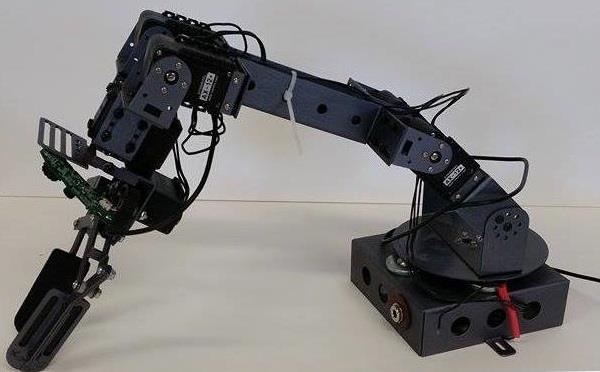
\includegraphics[width=10cm]{arm.jpg}
\end{center}
\caption{Previous Robotic Arm}
\label{fig:arm}
\end{figure}
\noindent
Previously Tiberius had a small arm, it could only lift about a kilogram and was very short, too short to reach the ground if mounted on Tiberius III.  
\subsection{Tiberius III's arm}
\subsubsection{Hardware}
In light of the problems of the old arm it was decided that a new arm would be designed that could lift a reasonably heavy object of about 2Kg from the ground in front of Tiberius and store it in a basket on the side of the robot.
\newline
The arm also had to be able to keep position without requiring power which required the use of worm drives for all joints. This would stop the arm from flailing around when not in use, since it would be a huge waste of power to keep it powered all the time. Additionally the use of worm drives gives a very large gear ratio with a simple design so makes the arm easier to design.

\subsubsection{Software}
The software consisted of several pieces of code working in combination.  The arm joints were controlled by stepper motors which required an accurate number of steps to translate to an angle.
The gripper was controlled by a servo which was stripped down to act as a simple motor.  
\newline
Consideration was given on how to implement the robotic arm, including ideas such as robotic software packages or libraries such as ROS, but eventually our own implementation was decided on.  This was partly due to the fact that the robotic arm was a customised arm made with 2 joints and a limited gripper capability.  These libraries were quite involved and would not fit easily into our Raspberry Pi controlled python code, additionally, a lot of examples of robotic arm had 3 or more joints and were structured quite differently so our own customised code would be the best option for controlling the arm.


\subsection{Gripper}
The gripper was designed by Y. Tlegenov, K. Telegenov, A. Shintemirov and released on an open source license. It was printed in 20 separate pieces of PLA and Nylon and then assembled.
This particular gripper was designed to use springs on each finger to allow the retraction of the hand to occur in the upper or lower part of the finger as necessary depending on the object being picked up.


\subsection{Camera}
It is inevitable that if the arm was to be controlled by teleoperation the robot would require a robust image capturing device with a clear view of the arm's area of operations. The Kinect 2 was situated to the front of the vehicle such that it provided a clear view perpendicular to the robot’s arm when it would try to grasp objects. A second camera was placed inside the gripper. The gripper camera allows the user to navigate the arm in the x and y axis and the Kinect 2 allows navigation in the z axis. 

